\section{Data Corpus and Graph Construction}
\label{sec:data_construction}
\subsection{Collection and Units}
The collector seeds a high-impact npm list, expands dependencies through deps.dev~\cite{depsdevapi}, requests registry metadata, and checks linked GitHub repositories for a \code{.github/workflows} directory at HEAD. Queue dates span June 13--16, 2026, but individual fields lack a common acquisition cutoff. The retained archive analyzed on October 20 contains 25,228 graph identifiers, 22,340 version-metadata rows, 12,217 maintainer usernames, and 79,405 package--maintainer relations. Maintainer membership is not a historical publisher log.

Among these identifiers, 2,745 encode bundled contexts rather than independently registered packages. The 121,885 retained version-edge rows project to 88,113 distinct name adjacencies. Stored \code{DIRECT}/\code{INDIRECT} labels describe a target node relative to an extraction root; their 48,705/73,180 row counts do not partition global direct and transitive edges~\cite{depsdevapi}. We reverse every explicit declaring-to-dependency adjacency to measure downstream reach.

\begin{figure*}[t]
\centering
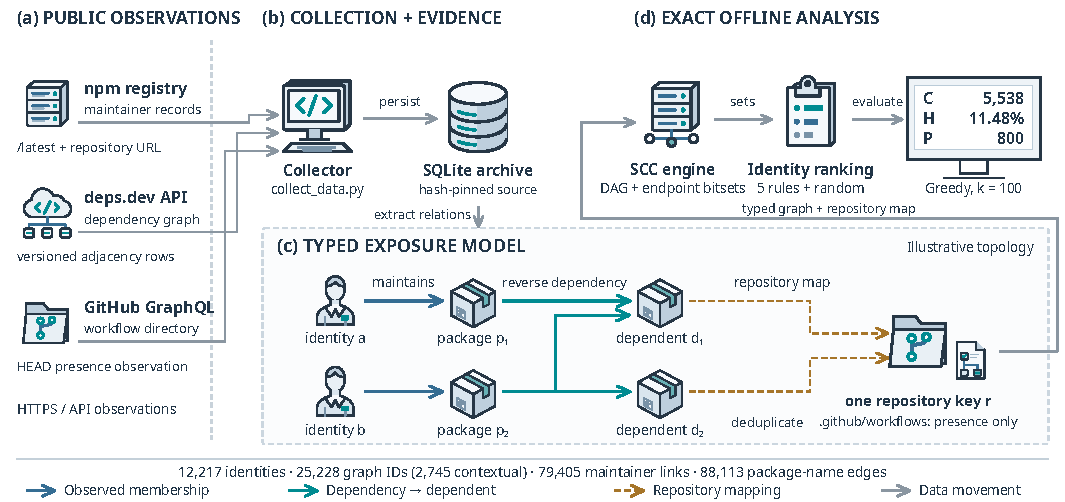
\includegraphics[width=0.96\textwidth]{study_system.pdf}
\caption{Implemented measurement architecture. Icons denote logical roles and topology is illustrative. Counts and displayed greedy outcomes are empirical; workflow presence does not establish execution.}
\label{fig:q1_observation_workflow}
\end{figure*}

The 15,233 workflow-positive package names map to 7,171 normalized repository keys. Owner/name pairs are case-folded and trailing transport \code{.git} is removed. This is lexical deduplication, without redirect or commit verification. There are 3,081 identifiers without maintainer mappings and 3,772 without completed workflow flags. Zero flags conflate directory absence with repository unavailability. Workflow endpoints require a positive observation; missing and zero flags are not evidence of safety. Coverage uses all 7,171 repository endpoints. Only 7,158 have an observed source identity; the other 13 are excluded from source-exclusion counts.

\begin{figure*}[t]
\centering
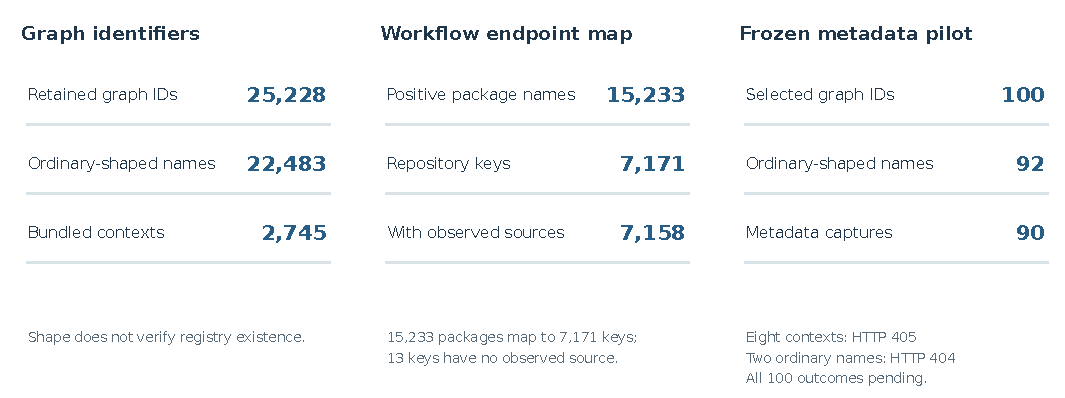
\includegraphics[width=0.94\textwidth]{observation_scope.pdf}
\caption{Observation units and prospective acquisition. Panels describe separate populations; their missingness counts must not be added across panels. Context identifiers are retained graph units, not separate registry packages. The prospective selection was frozen before requests; all 100 outcomes remain pending.}
\label{fig:q1_observation_scope}
\end{figure*}

Figure~\ref{fig:q1_observation_scope} separates graph units, observed workflow endpoints, and the prospective selection frame. This distinction matters because directory observation and metadata acquisition do not validate a historical installation or a future outcome.

\subsection{Name Projection and Exact-Version Continuity}
The name graph merges retained versions sharing an identifier. The sensitivity graph retains 40,806 exact (package, version) nodes and joins paths only at matching version keys. A maintained package seeds every retained version; without a version node, it contributes only its eligible seed endpoint. Both representations use the same package-level workflow flags. Neither reproduces npm installation or historical lockfile behavior: contexts and acquisition times remain mixed.

\begin{figure}[t]
\centering
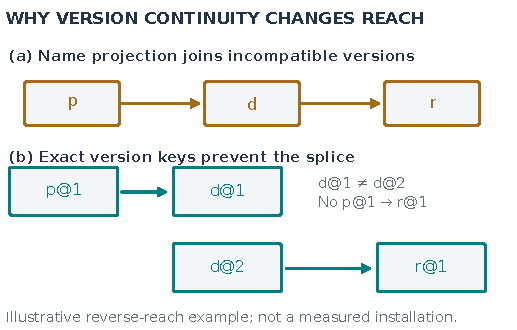
\includegraphics[width=\columnwidth]{graph_semantics.pdf}
\caption{Illustrative version splicing. Collapsing intermediate versions creates a name-level path without an exact-version counterpart. Reverse-reach arrows do not describe a measured installation.}
\label{fig:q1_version_semantics}
\end{figure}

\subsection{Cycles, Mapping Disagreements and Contexts}
The name graph has 82 nontrivial strongly connected components (SCCs) containing 403 nodes; the exact-version union has 68 containing 304 nodes. The largest component has 61 nodes in each. SCC condensation preserves reach and permits exact bitset propagation over a directed acyclic graph; the implementation uses arbitrary-precision Python integers, not fixed 64-bit sets. This is a computation technique, not an intervention that removes cycles.

The URL audit finds 658 identifier-level parser disagreements. Excluding 60 inconsistent positive observations reduces the workflow repository universe to 7,147; greedy at budget 100 gives $C=5{,}524$ and $P=799$. We discard ambiguous flags rather than transferring them to a corrected URL without reacquisition. Removing bundled-context nodes preserves all 462,170 primary account--repository incidences for fixed selections, although workflow-package incidence changes. That invariance does not apply automatically to every endpoint definition or individual-package ranking.
